% ----------- INTRODUCTION ---------- %
\chapter{Introduction}
\label{chapter:introduction} 
\noindent\rule{\linewidth}{2pt}

\section{Motivation}
In the present world, the use of advancing technology and application of Computer Science and Artificial Intelligence is growing drastically, especially in the biomedical sector for various purposes such as medical treatment, disease detection and diagnosis, etc. Artificial Intelligence has helped in reducing time consumed in diagnosis along with minimizing the scope of human errors. A sub-section of all the applications of Artificial Intelligence in Biomedical science is in Medical Image processing and disease diagnosis, i.e., the classification of diseases with minimal error. This technique utilizes various image processing techniques for smoothing, enhancement, colorization, and classification techniques. The scope of Artificial Intelligence in retinal disease classification has increased significantly with advancements in eye-imaging techniques and artificial intelligence making it useful for ophthalmologists to devise a better way of determining the probability of a disease and to provide an immediate treatment or cure. The use of Artificial Intelligence reduces the time taken to assess several patients significantly and efficiently.

\par
The images of retina, the back portion of the eye can be used to determine an ocular disease, if any. The light-sensitive layer at the rear of a human eye is called the retina. The retina has special cells called as photo-receptors which receives the image and sends it to the brain in the form of electric signals. There are two types of photo-receptor cells in retina: the rods, which detect low intensity light and cones, which are responsible for the detection of high intensity light or bright light. If the retina is affected or damaged, it may cause retinal diseases like Diabetic Macular Edema (DME), Central Serous Retinopathy (CSR), Macular Hole, Retinal Detachment, Age-related Macular Degeneration (AMD), etc. or complete vision loss. Artificial Intelligence uses medical images of the retina, processed, and enhanced using various image enhancement techniques for classification. 

\section{Optical Coherence Tomography}
To detect retinal diseases, we require a scan of the human eye. There are various imaging techniques that are used to study the human eye including Optical Coherence Tomography, Fundus photography, Fluorescent angiography, Ultrasound imaging, etc. Among these, Optical Coherence Tomography (OCT)\cite{OCT1991} is a non-invasive technique to capture the layers of retina with its features in very high resolution. It uses coherent light to capture 2-D or 3-D image of retinal structure. Unlike other imaging methods OCT can help to capture the depth features of the retina like retinal structure, tissue morphology to near microscopic resolution. It uses near-infrared light to penetrate the tissue to hundreds of micron depth and form a structural image. There are two distinct kinds of Optical Coherence Tomography based on the domain of measurements, the Time domain OCT (TD-OCT) and Spectral domain OCT (SD-OCT).

\begin{figure}[htb]
\centering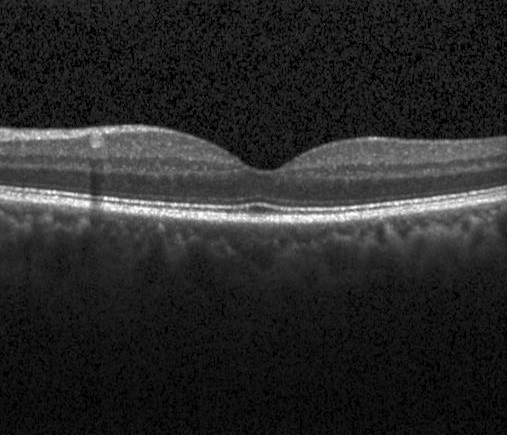
\includegraphics[width=0.5\linewidth]{figimages/Normal_eye.jpg}
\caption{OCT Scan of a Normal eye} 
\label{fig:OCT}
\end{figure}

\subsection{Time-domain Optical Coherence Tomography}
\vspace{1em}
In TD-OCT, the light beam gets divided into two parts: the sample beam and the reference beam. The retinal tissue gets struck by the sample beam and the light beam that is reflected after striking the tissue being imaged, is compared to the reference beam. The difference in time between the light beams and the intensity of the reflected light is used to visualize the retinal structure and its layers.

\subsection{Spectral-domain Optical Coherence Tomography}
\vspace{1em}
In SD-OCT, the light beams are split in a similar manner into the reference beam and sample beam. However, in SD-OCT, it is preferred to use a light source that can emit light with a broad range of spectrum. The sample beam is directed towards the retina tissue. The beam reflected after striking the tissue being visualized, is analysed using a spectrometer. The spectrometer measures the intensity and wavelength of the reflected light, and is used to visualize a 3-D image of the retinal structure and its layers. Out of the two measurement methods, the SD-OCT is found to be faster and better compared to conventional TD-OCT method. 

\section{Retinal Diseases}
There are many retinal diseases which can be detected using OCT scans. Some of the diseases are central serous retinopathy, macular hole, age-related macular degeneration (AMD), drusen, etc.\cite{OCTdiseases} The diseases which are being considered for classification in this research work are described in a detailed manner in the following sections:

\subsection{Age-related Macular Degeneration}
\vspace{1em}
AMD is an ocular condition which occurs at old age. AMD occurs at a much slower rate as compared to other retinal diseases. AMD has the following two types:
\begin{enumerate}
    \item \textbf{Dry AMD:} In dry AMD, the central region of retina, macula, gets thinner with age and slowly the person loses their central vision. This creates a blind spot at the centre of the eye.
    \item \textbf{Wet AMD:} In wet AMD, blood vessels grow abnormally under the retinal layer which causes fluids to leak, damaging the macula. Wet AMD is severe compared to dry AMD as it can cause complete loss of vison. Also, Wet AMD develops far more quickly than dry AMD.
\end{enumerate}

\begin{figure}[htb]
\centering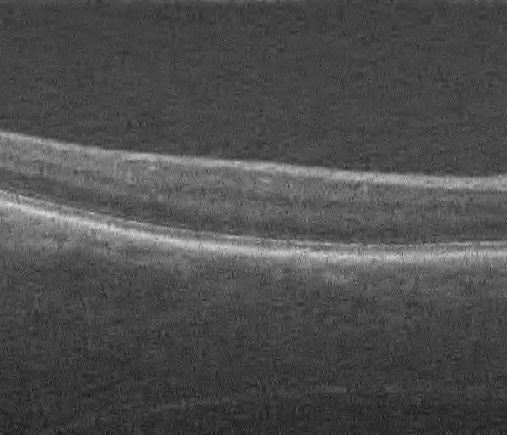
\includegraphics[width=0.5\linewidth]{figimages/AMD.jpg}
\caption{Age-related Macular Degeneration (AMD)} 
\label{fig:AMD}
\end{figure}

\subsection{Central Serous Retinopathy}
\vspace{1em}
CSR is the ocular disease in which fluids from choroid tissue layer leaks under the retina. It separates the retinal layer due to the cavity created, which causes blurry or unclear vision. CSR resolves usually in few months. Otherwise in some cases it may require medical attention.

\begin{figure}[htb]
\centering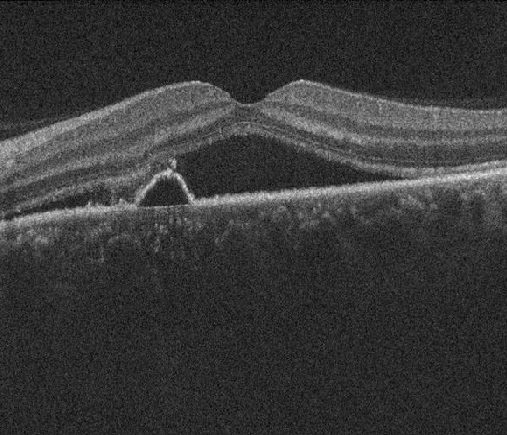
\includegraphics[width=0.5\linewidth]{figimages/CSR.jpg}
\caption{Central Serous Retinopathy (CSR)} 
\label{fig:CSR}
\end{figure}

\subsection{Macular Hole}
\vspace{1em}
When a tear is formed at macula due to being forced or stretched, the central vision of the eye blurs. This condition is called Macular Hole. Usually, macular hole is formed in the eyes with old age. The vitreous gel, which is the substance, which is filled between the lens and retina, wears off causing a macular hole to be generated.

\begin{figure}[htb]
\centering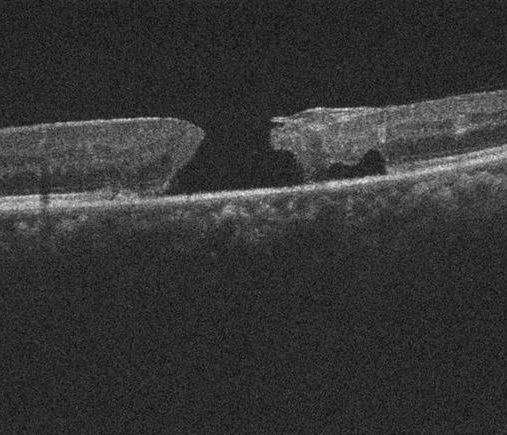
\includegraphics[width=0.5\linewidth]{figimages/MH.jpg}
\caption{Macular Hole} 
\label{fig:MH}
\end{figure}

\subsection{Drusen}
\vspace{1em}
Another ocular condition, Drusen is the deposition of yellow-coloured proteins and lipids or other waste materials under the retina. It may result in AMD, if left untreated. There are two types of Drusen:
\begin{enumerate}
    \item \textbf{Hard Drusen:} smaller particle deposits are termed as hard drusen. They do not in turn cause Age-related Macular Degeneration.
    \item \textbf{Soft Drusen:} large substances present in the eye are termed as soft drusen. They are related to Age-related Macular Degeneration.
\end{enumerate}
\begin{figure}[htb]
\centering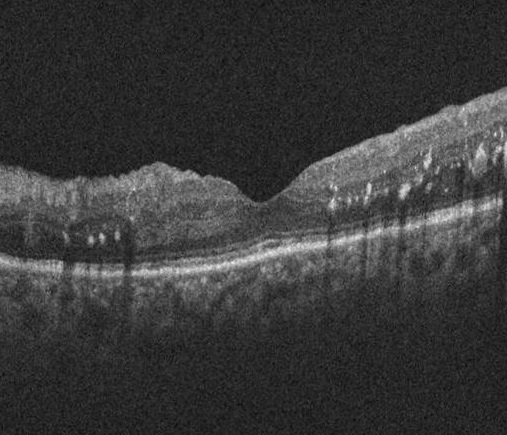
\includegraphics[width=0.5\linewidth]{figimages/Drusen.jpg}
\caption{Drusen} 
\label{fig:drusen}
\end{figure}

\section{Deep Learning}
Artificial Intelligence (AI) is the ability of computer systems or machine to mimic the human behaviour to identify or predict certain results including voice recognition, visual perception, prediction, etc. New advancements of modern age have found the use of AI at the centre of most of the industries. AI has various sub-domains including Natural Language Processing (NLP), Machine Learning, Robotics, etc.

\par
Machine learning is a sub-domain of AI which involves developing various algorithms which can predict certain outputs or classify inputs into different classes after training over given data. The main task of machine learning is to train the algorithms on data to learn and improve its performance. A typical machine learning task involves feature extraction from the given data, which is used in the algorithm as input to classify or predict the output. K-NN, Random Forest, Support Vector Machine (SVM) are few algorithms that have been used widely in Machine Learning.

\par
With new advancements, Deep Learning, which is a sub-field of machine learning has taken over and is being used for complex problems such as voice recognition, image classification, natural language processing etc. Deep Learning algorithms unlike machine learning, have complex multi-layered neural network structure which can automatically recognize patterns and features from the given raw data and provide a much higher accuracy as compared to the conventional methods. Deep learning algorithms may not require feature extraction step. The distinction between a machine learning and deep learning process is shown in Figure \ref{fig:machinedeeplearning}.

\begin{figure}[htb]
\centering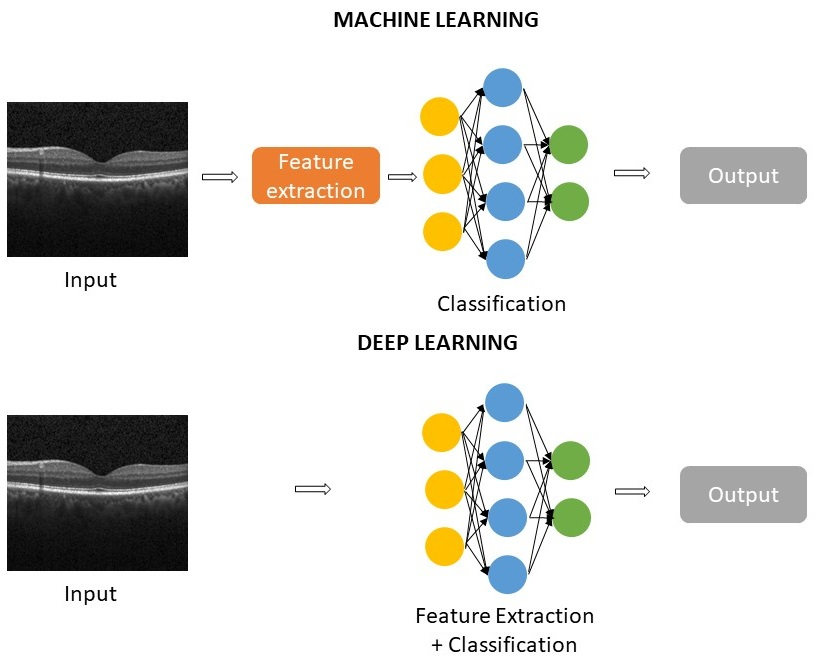
\includegraphics[width=0.85\linewidth]{figimages/Machine_Deep_Learning.jpg}
\caption{Comparison of Machine Learning and Deep Learning approaches} 
\label{fig:machinedeeplearning}
\end{figure}

\par
The use of Deep Learning for Artificial Intelligence problems has increased significantly in the past years with the rise in the access of more data and with increase of computational power. Graphical Processing Units (GPU) have been introduced, which is a type of processor which is used for complex calculations and parallel computations. The conventional machine learning training is carried out on CPU which is slower as compared to GPU computation speed.

\par
There are various types of deep learning network architectures which are designed to produce outputs specific to different set of problems. Two of the architectures which are important to this research work are described below:
\begin{enumerate}
    \item \textbf{Convolutional Neural Networks:} The CNN is a neural network architecture which is based on supervised learning, used mainly for classification tasks. A typical CNN consists of various layers including convolutional layers which are designed to extract image characteristics by sliding a kernel over image and create a different representation at each level, followed by other layers like pooling layers, batch normalization layers, and fully connected layers. The main advantage of using CNN over conventional machine learning method for classification is that CNN can learn the features and predict the class using raw image, whereas machine learning requires feature extraction before training to get better results.
    \item \textbf{Autoencoders:} Autoencoders \cite{Bank2020} are a specific type of neural network created to provide encoding and decoding of a given input to a desired form of output. Autoencoders are used for unsupervised learning problems including noise removal, reduce size to a smaller representation, automatic image colorization \cite{Singh2022}, etc. The Convolutional Autoencoders are a type of Autoencoders made using sequential convolutional layers for encoding and decoding of the input data. Zhang Y. \cite{Zhang} argued the use of Convolutional Autoencoders is best suited for images rather than linear autoencoders in their work. They compared the denoising and compression results of a convolutional and simple autoencoder in which the convolutional autoencoder outperformed the simple autoencoder. There are various use cases of Autoencoders out of which the Convolutional Autoencoders are mainly used for noise removal from images as shown in the research work by Yasenko \cite{DESSERT2020}. The Convolutional Autoencoders are trained with the actual image as the desired output and a slightly noisy image as the input. The autoencoder is trained with these input and output targets to provide a noise free output for a given image.
\end{enumerate}
\textbf{Hyperparameters:} Hyperparameters can be described as the changeable values in a deep learning training task which affects the algorithm and the results significantly. Hyperparameters are not learned by the algorithm but are provided or manually set by the user. It is necessary to choose the hyperparameter values carefully to obtain better result. Some of the hyperparameters are:
\begin{itemize}
    \item \textbf{Batch size:} Batch size is the number of training inputs which are fed in one iteration during training followed by weights updation. As the batch size increases, the convergence rate increases, however it requires a larger memory for computation. It is advised to start with a smaller batch size. \\
    With the decided batch size and size of input data, the total iterations per epoch is calculated.
    \begin{equation}
    \text{iterations} = \frac{\text{number of input data points}}{\text{batch size}}        
    \end{equation}
    \item \textbf{Epochs:} Epochs is each step of training, i.e., the number of times the training will loop over the data again and again to update the weights. In one epoch, the whole data is fed through the model and weights are updated, which is repeated in the next epoch. 
    
    \item \textbf{Loss Function:} It is a function which determines the overall loss a machine learning model makes during output prediction. It is calculated as the difference between the predicted and the true output. It is used to guide the optimizer algorithm to find the optimum value of weights which can achieve the minimum value of the loss function. The choice of loss function is specific to the given task. There are various loss functions including: \\
    Mean Square Error (MSE) Loss Function: MSE is generally used in regression tasks. It is the average squared difference between the predicted and the true output values.
    \begin{equation}
    MSE = \frac{1}{n}\sum_{i=1}^{n}(y_i - x_i )^2    
    \end{equation}
    where $y_i$ and $x_i$ are predicted and true output respectively. 

    Cross-entropy Loss Function: Similarly, the cross-entropy loss is used for classification tasks. It is the measure of difference between predicted probabilities and the true probabilities of the classes. It is calculated as
    \begin{equation}
        \text{Cross-entropy} = -\sum_{i=1}^nq_{i}\log(p_{i})
    \end{equation}
    where $q_i$ and $p_i$ are predicted and true probability respectively. 

    \item \textbf{Learning Rate:} It is the value which estimates the size of steps in which the weights are updated, or the step size with which the model converges. It is advised to begin with a small learning rate as a bigger value can cause the algorithm to overshoot and diverge from the minimum value. A smaller learning rate may increase the time of training but will reach an optimum value.
    
    \item \textbf{Optimizer:} Optimizer are the algorithm responsible for updating weights of a model during training step. The optimizer selected describes the way with which the weights will be updated to minimize the loss function. It works on the principle of back propagation. The simplest and most popular back propagation optimizer algorithm is Gradient Descent algorithm, also called as Stochastic Gradient Descent.

    \par
    Stochastic Gradient Descent (SGD): It modifies the model parameters according to the loss function gradient relative to the model parameters. It has a disadvantage, as it can get stuck in a local minimum and may fail to achieve the actual global minima.

    \par
    There are other optimizer algorithms available to overcome this and provide better results. Some of them are Adam optimizer, AdaGrad optimizer, RMSProp optimizer etc.
\end{itemize}

\section{The Process Flow of the Dissertation}
The following is the progression of this dissertation, through which the success of this work is achieved:

\begin{enumerate}
    \item \textbf{Chapter \ref{chapter:introduction} Introduction:} This is the introductory chapter of this dissertation. It explains the need of growing use of Artificial Intelligence in various sectors and its demand in medical sciences. It explains OCT, an optical scanning technique which is used for identification of various retinal diseases including Macular Hole, Age-related Macular Degeneration (AMD), Central Serous Retinopathy (CSR), and Drusen. It also sheds some light on the various AI methods involved in the research work like CNN, Autoencoders, and discuss various algorithms and hyperparameters and their importance that are involved in the training of these deep learning networks. 
    
    \item \textbf{Chapter \ref{chapter:literature} Literature Survey:} This chapter discusses various research and work that has been carried out in this field and which aligns with the research objectives. Additionally, it provides an insight on various methods that have been deployed or improved in this dissertation. The results of various methods have been obtained from this section to compare with the work in this dissertation.
    
    \item \textbf{Chapter \ref{chapter:proposedWork} Proposed Work:} This chapter discusses the methodology proposed in this research work. The research proposed utilizes a large collection of OCT images of each of these ocular conditions and develops a classifier to accurately classify the normal eye, and four other ocular diseases or conditions. The OCT images are processed and fed to a Convolutional Autoencoder network for noise removal. The denoised images are then enhanced or adjusted using Contrast Limited Adaptive Histogram Equalization (CLAHE).The enhanced images are normalized using the mean and standard deviation values. The image data is then trained on two different Convolution Neural Network (CNN) models. The first architecture is a simple CNN of five layers, and the other, a novel architecture, which utilizes bottleneck layer structures with convolutional layers. The purpose of this study is to enhance the existing detection method of diseases and provide a more efficient method for the ophthalmologists to utilize.
    
    \item \textbf{Chapter \ref{chapter:results} Experiments and Results:} In this chapter, the training and testing phase of the work is discussed. The training process is described along with the evaluation results obtained. Various evaluation parameters like Mean Square Error (MSE), Peak Signal-to-Noise Ratio (PSNR), Training and Validation Accuracy, Recall, Confusion matrix, F1 Score, etc. are used to evaluate the deep learning models’ performance. The training plots have also been visualized for the proposed methods.
    
    \item \textbf{Chapter \ref{chapter:conclusion} Discussion and Conclusion:} This chapter provides a comparison of the proposed method with the previous methods and its advantages over the previous approaches. It also concludes the research work. 
\end{enumerate}

% ------------------------ END -----------------------%